%% Documentclass:
\documentclass[manuscript]{stjour}

%% Or,

%% Manuscript, for double spaced, larger fonts
% \documentclass[manuscript]{stjour}
%% Only needed if you use `manuscript' option
% \journalname{Open Mind}

%%%%%%%%%%%%%%%%%%%%%%%%%%%%%%%%%%%%%%%%%%%%%%%%%%
%% For production only, not authors:
%%\documentclass[OpenMind,finalfonts]{stjour}

%%%%%%%%%%% Please supply information %%%%%%%%%%%%%%%%%%%%%%%%%

%% For Open Mind:
%% Supplementary Materials:
\supplementslinks{dx.doi.org/10.1098/rsif.2013.0969}

%% If no conflicts, this command doesn't need to be used
%% \conflictsofinterest{}

%%%%%%%%%%% to be supplied by MIT Press, only %%%%%%%%%%%%%%%%%

\citation{Niyogi, R. K., Breton, Y.-A., Solomon,
R. B., Conover, K.,\\ Shizgal, P., Dayan, P. (2015).\\ 
Optimal indolence: a normative microscopic approach to work and leisure. Open Mind 1(1):
1−12.}

\received{20 October 2013}
\accepted{7 November 2013}
\published{26 January 2014}

%% DOI address:
\setdoi{10.1098/rsif.2013.0969}

%%%%%%%% End MIT Press commands %%%%%%%%%%

%%%%%%%%%%%%%%%%%%%%%%%%%%%%%%%%%%%%%%%%%%%%%%%%%%%%%%%%%%%%%%%
%% author definitions should be placed here:

%% example definition
\def\taupav{\tau_{\mathrm{Pav}}}
\begin{document}

\title{Convention formation through local language acquisition}
\subtitle{<Subtitle Here>} %% Optional subtitle

%% If shortened title for running head is needed so that the article title can fit
%%   in the running head, use [] argument, ie,
%%
%%   \title[Shortened Title for Running Head]{Title of Article}
%%   \subtitle{Subtitle Here}

%%% Author/Affil
%% Since we use \affil{} in the argument of the \author command, we
%% need to supply another version of the author names, without \affil{}
%% to be used for running heads:

\author[Author Names]
{Robert Hawkins, Mike Frank, Noah Goodman\thanks{<for footnote for further info>}\affil{1}}

\affiliation{1}{Department of Psychology, Stanford University, Stanford, CA, US}

%ie
%\affiliation{2}{Center for Studies in
%Behavioral Neurobiology, Concordia University, Montreal, Quebec,
%Canada}

\correspondingauthor{Robert Hawkins}{rxdh@stanford.edu}

% ie,
%\correspondingauthor{Ritwik K. Niyogi}{ritwik.niyogi@gatsby.ucl.ac.uk}

\keywords{conventions; pragmatics; communication; learning}

%ie
%\keywords{work, leisure, normative, microscopic,  reinforcement learning, economics}

\begin{abstract}
What cognitive mechanisms support the emergence of linguistic conventions from repeated interaction? We present results from a large-scale, multi-player replication of the classic tangrams task which demonstrate three key empirical signatures constraining theories of convention-formation: arbitrariness, stability, and reduction of utterance length over time. These results motivate a theory of convention-formation where agents, though initially uncertain about word meanings in context, assume others are using language with such knowledge. Thus, agents may learn about meanings by reasoning about a knowledgeable, informative partner; if all agents engage in such a process, they successfully coordinate their beliefs, giving rise to a conventional communication system. We formalize this theory in a computational model of language understanding as social inference and demonstrate that it produces all three signatures.
\end{abstract}

\section{Introduction}\label{introduction}

Just as drivers depend on shared behavioral conventions to safely
navigate traffic, successful communication depends on a set of shared
linguistic conventions. Speakers of different languages around the world
refer to the same object in many different ways, yet when ordering a
coffee in San Francisco, I can confidently use the English word
``coffee'' and assume that I will be understood. How do these
conventions -- classically characterized by Lewis (1969) as arbitrary
but stable solutions to recurring coordination problems -- form in the
first place?

While \emph{global} conventions adopted and sustained throughout a large
population of speakers may develop over longer time scales, we also
effortlessly coordinate on \emph{local} conventions -- or conceptual
pacts (Brennan \& Clark, 1996) -- within the span of a single dialogue.
For example, when discussing possible conditions to use in an upcoming
experiment, a team of collaborators might begin the meeting using long
descriptions to refer to each condition but end the meeting using
conventional terms like ``condition A'' and ``condition B.'' Since
global conventions are hypothesized to emerge through diffuse, repeated
interactions of this more local kind (Garrod \& Doherty, 1994), the
cognitive mechanisms underlying convention-formation in such games are
of foundational interest.

In a seminal study by Krauss \& Weinheimer (1964), pairs of participants
played a cooperative language game where they were presented with arrays
of ambiguous shapes in randomized orders. The players were assigned the
roles of \emph{director} and \emph{matcher} and allowed to talk freely.
The matcher's goal was to rearrange their shapes to match the director's
board, and the director's goal was to communicate useful descriptions.
Over multiple rounds, descriptions were dramatically shortened: an early
description like ``upside-down martini glass in a wire stand,'' became
simply ``martini'' by the end. Later studies (e.g. Clark \&
Wilkes-Gibbs, 1986) refined this paradigm, using larger arrays of
tangram-like figures and emphasizing the intricate back-and-forth
process through which speakers and listeners negotiate over references.
These studies revealed a number of key empirical signatures that inform
theories of convention-formation. Here, we focus on three:
arbitrariness, stability, and the systematic reduction of utterance
length over time.

\emph{Arbitrariness} is a definitional property of conventions (Lewis,
1969): there must be multiple solutions that would be equally successful
as long as both players ``agree'' (e.g.~driving on the left vs.~right
side of the road). By the final round in a language game, for example,
the same tangram might be called the `dancer' to one pair and the
`skater' to another. The other definitional property we consider is
\emph{stability}: it is in everyone's best interest to keep using the
convention, once established. Finally, \emph{reduction} is more specific
to the reference game paradigm and refers to the transformation of
longer, complex expressions into simpler expressions over the course of
interaction, as Krauss \& Weinheimer (1964) observed. While this broad
phenomenon has been replicated many times, exactly what is reduced
remains an open empirical question.

Theories of convention-formation differ primarily in the extent to which
sophisticated social reasoning and common ground is required. At one
extreme, agents use simple heuristic updating rules and do not need to
represent or reason about other agents at all (Barr, 2004; Centola \&
Baronchelli, 2015; Young, 2015). Simulations elegantly show how
arbitrary signaling systems can spread and come to dominate large
populations. However, due to their `rich get richer' dynamic, it is not
clear how emergence-through-use mechanisms alone could account for
reduction in repeated interaction. At the other extreme, are theories in
which agents explicitly consider their partner's beliefs and track what
information is \emph{mutual knowledge}, often formalized in a game
theoretic setting (Lewis, 1969). Wilkes-Gibbs \& Clark (1992) and others
have proposed that agents engage in a collaborative process of
establishing mutual knowledge, though the mechanisms allowing
conventions to emerge under such conditions have not been instantiated
in a formal model to our knowledge.

In this paper, we argue for a theoretical position on the spectrum
between these poles: \emph{conventions form when agents assume
conventions already exist}. In other words, agents believe there is a
true lexicon used by other agents but are initially unsure of its
identity. Through their interactions with a partner who is assumed to be
knowledgeable and informative, agents can learn this true lexicon even
though their partner in fact begins in the same state of ignorance.
Agents thus coordinate on the same lexicon, which becomes conventional.

To support this theory, we first conduct a large-scale, multi-player
replication of the tangrams task, which has traditionally been limited
to relatively small sample sizes in the lab. We demonstrate signatures
of arbitrariness, stability, and reduction which have been difficult to
study at a fine-grained level due to the sparseness of existing data.
Next, we formulate our theory in a computational model of communication
in repeated reference games, based on recent successes capturing
language understanding as social inference (Goodman \& Frank, 2016;
Goodman \& Stuhlmüller, 2013) and show that this model qualitatively
produces all three empirical signatures.

\section{Replication of tangrams
task}\label{replication-of-tangrams-task}

To collect a corpus of reference game dialogue that supports more
detailed analyses of convention-formation, we ported the tangrams task
used in Clark \& Wilkes-Gibbs (1986) to a real-time, multi-player web
environment.

\subsection{Methods}\label{methods}

\subsubsection{Participants}\label{participants}

200 participants were recruited from Amazon's Mechanical Turk and paired
into dyads to play a real-time communication game using the framework in
Hawkins (2015). We excluded games that terminated before the completion
of 6 rounds and where participants reported a native language different
from English, leaving a corpus of X complete games with a total of
Xutterances.

\subsubsection{Stimuli}\label{stimuli}

On every trial of the game, both participants were shown a
\(6 \times 2\) grid containing twelve tangram shapes, reproduced from
Clark \& Wilkes-Gibbs (1986). Cells were labeled with fixed numbers from
one to twelve in order to help participants easily refer to locations in
the grid (see Fig. \ref{fig:taskScreenshot}).

\subsubsection{Procedure}\label{procedure}

After passing a short quiz about task instructions, participants were
randomly assigned the role of either `director' or `matcher' and
automatically paired into virtual rooms containing a chat box and grid
of stimuli. Both participants could freely use the chat box to
communicate at any time. The director's tangrams were fixed in place,
but the matcher could click and drag the shapes to reorder them. The
director had to send messages about the locations of different tangrams
on their fixed board (e.g. ``\#1 looks like an X'', ``2 is the one with
the Y''); the matcher had to identify the corresponding tangram shapes
and move them to the correct locations. When the players were satisfied
that their boards matched, the matcher clicked a `submit' button that
gave players feedback on their score (out of 12) and scrambled the
tangrams for the next round. After six rounds, players were redirected
to a short exit survey. We collected the raw text of every message sent
and every swapping action taken by the matcher.

\subsection{Results}\label{results}

\subsubsection{Arbitrariness and
stability}\label{arbitrariness-and-stability}

We begin by examining signatures of \emph{arbitrariness} and
\emph{stability} in our data. We operationalize these concepts using the
information-theoretic measure of entropy:
\[H(W) = \sum_w P(w) \log P(w)\] Broadly speaking, entropy measures the
predictability of a distribution. It is maximized when all elements are
equally likely and declines as the distribution becomes more structured,
i.e.~when the probability mass is concentrated on a subset of elements.

To derive predictions, we consider a permutation-test null model in
which utterances are scrambled within each round. The empirical entropy
of individual games should only differ from the null distribution if
\emph{both} arbitrariness and stability hold. First, note that if
stability did \emph{not} hold, scrambling would have no effect on the
entropy within individual games: speakers would already use different
words each round, and swapping out the identity of those words would not
affect the entropy of the word distribution.

If stability holds but arbitrariness does not, all players would adopt
the single optimal (non-arbitrary) way to refer to each tangram.
Therefore, the entropy of their word distributions also should not be
affected by scrambling: a speaker's real words would be swapped out for
the same words, just generated by another speaker. Finally, if both
arbitrariness and stability hold, then different speakers adopt
different referring expressions that persist from round to round. Hence,
scrambling should \emph{increase} the average game's entropy from a
relatively low level: each game's idiosyncratic, concentrated
distribution of words would be mixed together to form more heterogeneous
and therefore high-entropy distributions.

To test this prediction, we computed the average within-game entropy for
1000 different permutations of speaker utterances. We permuted
utterances within rounds rather than across the entire data set to
control for the fact that earlier rounds have longer utterances and thus
a larger vocabulary than later rounds (see the following section). Since
this permutation scheme keeps the number of messages per participant
constant and simply swaps out the content of those messages, it also
controls for the fact that some speakers sent more messages than others.
We found that our null distribution lay within the interval {[}X, Y{]},
which is significantly higher than the true entropy (averaged across
games) of Z \(p < 0.001\). This pattern is consistent only with
signatures of both arbitrariness and stability.

\subsubsection{Reduction}\label{reduction}

Next, we turn to a set of analyses examining reduction in utterance
length over the course of the experiment. At the coarsest level, we find
that the mean number of words used by speakers decreases over time (see
Fig. \ref{fig:replication}). This decrease replicates a highly reliable
reduction effect found throughout the literature on iterated reference
games (Brennan \& Clark, 1996; Krauss \& Weinheimer, 1964), although
perhaps due to our purely textual (vs.~spoken) interface, participants
in our task used many fewer words overall than previously reported. The
following analyses break down this broad reduction into a finer-grained
set of phenomena.

The next level of granularity motivating our model approach concerns
which kinds of words are most likely to be dropped. Is the speaker
adopting a shorthand where they drop uninformative function words, or
are they simplifying or narrowing their descriptions by omitting
meaningful details (Clark \& Wilkes-Gibbs, 1986)? We used the Stanford
CoreNLP part-of-speech tagger (Toutanova, Klein, Manning, \& Singer,
2003) to count the number of words belonging to each part of speech in
each message. Fig. \ref{fig:pos} shows the percent reduction of
different parts of speech from the first round to the sixth round. We
find that determiners (`the', `a', `an') are the most likely class of
words to be dropped with an X\% reduction rate, on average. Nouns
(`dancer', `rabbit') are the least likely class to be dropped with only
an Y\% rate. Closed-class parts of speech are strictly more likely to be
dropped than open-class parts of speech.

While this finding suggests that speakers might just be adopting a
shorthand using more ungrammatical fragments as the game proceeds, we
find a more complex dynamic by examining the table of unigrams and
bigrams most likely to be dropped (see Table \ref{tab:words}). Note that
alongside dropped articles, there are a number of words that form
conjunctions (`and') and modifiers (`of', `with', `the right'). In other
words, it may be more likely that when function words are dropped, it is
primarily as part of larger grammatical units that provide additional
information in identifying the target.

We explicitly examined this hypothesis by running the Stanford
constituency parser (Schuster \& Manning, 2016), tagging the occurrence
of subordinate/adverbial clauses (`sitting \emph{facing left}') and
adjectival clauses (`angel \emph{that is praying}').\footnote{Specifically,
  we used the Universal Dependencies tags \texttt{csubj, ccomp, xcomp},
  and \texttt{advcl} for subordinate clauses and \texttt{acl} for
  adjectival clauses (Schuster \& Manning, 2016)} We found that both
were reduced over the course of the game (see Fig.
\ref{fig:replication}), lending additional support for the hypothesis
that meaningful details are increasingly omitted. Initial phrases pile
on multiple ambiguous, partially redundant modifiers and descriptors: as
the game progresses and ambiguity of reference decreases, these
additional meaningful units become less useful and can be dropped.

\subsubsection{Listener feedback}\label{listener-feedback}

Finally, the theory proposed by Clark \& Wilkes-Gibbs (1986) argues that
lexical conventions are established through a collaborative process
requiring both speaker and listener input. This predicts that (1)
listener feedback should be highest on the first round and drop off once
meanings are agreed upon, and (2) dyads with more initial listener
feedback should converge on more efficient conventions. We find
correlational evidence of both patterns in our data. The number of
listener messages decreases significantly over the game (\(t = -13.23\),
see Fig. \ref{fig:replication}), and there is a weak but significant
effect of initial listener messages on overall reduction (X).

\section{Model}\label{model}

Here, we present a probabilistic model of language production under
uncertainty, which captures several of the signature properties of
conventions shown above. This model belongs to the family of Rational
Speech Act (RSA) models, which have been successful in explaining a wide
range of linguistic phenomena -- including scalar implicature,
adjectival vagueness, overinformativeness, indirect questions, and
non-literal language use -- as arising from a process of recursive
social reasoning. Most previous applications of RSA have focused on the
listener's problem of language comprehension, but the puzzle of
conventionalization is primarily a question of speaker production. An
\(n\)th order pragmatic speaker trying to convey a particular state of
affairs \(s \in \mathcal{S}\) assuming lexicon \(\mathcal{L}\) is
assumed to select an utterance \(u \in \mathcal{U}\) by trading off its
expected informativity (with respect to a rational listener agent)
against its cost, usually based on length (Goodman \& Frank, 2016):
\[S_n(u | s, \mathcal{L}) \propto \exp{\left(\alpha \log L_n(s | u, \mathcal{L}) - \textrm{cost}(u)\right)}\]
where \(\alpha\) is an optimality parameter controlling the extent to
which the speaker maximizes over the expected listener distribution. The
listener, in turn, reasons about what utterances would be most likely to
be produced by a speaker intending to convey \(u\):
\[L_n(s | u, \mathcal{L}) \propto P(s) S_{n-1}(u | s, \mathcal{L})\]
\indent This recursion bottoms out in a \emph{literal listener} who
directly looks up the meaning of the utterance in the lexicon:
\[L_0(s | u, \mathcal{L}) \propto \mathcal{L}(u, s)\cdot P(s)\]
\indent As in several other recent applications of RSA (Graf, Degen,
Hawkins, \& Goodman, 2016), we use a graded semantics, where utterances
are better or worse descriptions of particular referents. For instance,
the utterance ``dancer'' may initially be expected to apply to a
photorealistic image of a ballerina
(\(\mathcal{L}(\textrm{'dancer'}, \textit{ballerina}) = 0.99\)) more
than an abstract image of one
(\(\mathcal{L}(\textrm{'dancer'}, \textit{abstract ballerina}) =0.6\)),
but apply to both better than a non-category member like an image of a
dog (\(\mathcal{L}(\textrm{'dancer'}, \textit{dog}) = 0.05\)).

Our approach to convention-formation begins with the additional
assumption of \emph{lexical uncertainty} (Bergen, Levy, \& Goodman,
2016; Smith, Goodman, \& Frank, 2013). In other words, we assume that
instead of having perfect knowledge of \(\mathcal{L}\), the speaker has
uncertainty over the exact meanings of lexical items in the current
context (i.e.~it is initially unclear which of the ambiguous tangram
shapes ``the dancer'' might refer to). They begin with some prior
\(P(\mathcal{L})\) over meanings, which may be initially biased toward
certain meanings, and update these beliefs through repeated interactions
with a knowledgeable partner:
\[P(\mathcal{L} | d) \propto P(\mathcal{L})\prod_i L_{n-1}(s_i|u_i, \mathcal{L})\]
where \(d = \{s_i, u_i\}\) is a set of observations of \(s_i\) and
\(u_i\) coming from previous exchanges\footnote{There is a broader
  debate over the timescales at which lexicons and lexicon learning
  mechanisms operate; here, we assume a discourse-level structure to the
  lexicon, where there is uncertainty over how words are used \emph{in
  the given conversation}. See Frank, Goodman, \& Tenenbaum (2009) for a
  related approach at the scale of cross-situational word learning.}.
The speaker then marginalizes over this posterior distribution when
reasoning about the listener, giving rise to the form of the pragmatic
listener model we use throughout our model results (only going up to
\(n = 2\) in our recursion for simplicity):
\[S(u | s, d) \propto \exp( \alpha\log\left(\sum_{\mathcal{L}} P(\mathcal{L} | d) L_1(s | u, \mathcal{L})\right) - \textrm{cost}(u) )\]
\indent A listener with lexical uncertainty can be defined similarity,
simply swapping out \(L_{n-1}\) in the lexicon posterior update with a
knowledgeable speaker \(S_{n}\):
\[L(s | u, d) \propto \sum_\mathcal{L}P(\mathcal{L}|d)L_1(s|u,\mathcal{L})\]
\indent This model is implemented in the probabilistic programming
language WebPPL (Goodman \& Stuhlmüller, electronic).\footnote{All
  results can be reproduced running our code in the browser at
  \url{http://forestdb.org/models/conventions.html}} Following Smith et
al. (2013), we begin by showing how a random initial choice is taken to
be evidence for a particular lexicon and becomes the base for successful
communication even though neither party knows its meaning at the outset.

\subsection{Results}\label{results-1}

\subsubsection{Arbitrariness and
stability}\label{arbitrariness-and-stability-1}

Consider an environment with two abstract shapes (\(\{s_1, s_2\}\)),
where the speaker must choose between two utterances (\(\{u_1, u_2\}\))
incurring equal cost. Their prior \(P(\mathcal{L})\) over the meaning of
each utterance is given by a (discretized) Dirichlet distribution, so on
the first round both utterances are equally likely to apply to either
shape. If the speaker was trying to get their partner to pick \(s_1\),
then, since each utterance is equally (un)informative, they would
randomly sample one (say, \(u_1\)), and observe the listener's selection
of a shape (say, \(s_1\)). On the next round, the speaker uses the
observed pair \(\{u_1, s_1\}\) to update their beliefs about the
lexicon, uses these beliefs to generate a new utterance, and so on. To
examine expected dynamics over multiple rounds, we enumerate over all
possible trajectories our simulated speaker and listener models could
produce.

We observe several important qualitative effects in our simulations.
First, the fact that a knowledgeable listener responds to utterance
\(u\) with \(s\) provides evidence for lexicons in which \(u\) is a good
fit for \(s\), hence the likelihood of the speaker using \(u\) to refer
to \(s\) increases on subsequent rounds (see
Fig.\ref{fig:modelConvergence}). In other words, the initial symmetry
between the meanings can be broken by initial random choices, leading to
completely \emph{arbitrary but stable mappings} in future rounds.
Second, because the listener is also learning the lexicon from these
observations under the same set of assumptions, they converge on a
shared set of meanings; hence, expected \emph{accuracy} rises on future
rounds (see Fig. \ref{fig:modelAcc}). Third, because one's partner is
assumed to be pragmatic, agents can also learn about \emph{unheard}
utterances: observing \(\{u_1, s_1\}\) also provides evidence for
lexicons in which \(u_2\) is a good fit for \(s_2\) by standard Gricean
reasoning. Finally, \emph{failed references} lead to conventions just as
effectively as successful references: if the speaker intends \(s_1\) and
says \(u_1\), but then the listener incorrectly picks \(s_2\), the
speaker will take this as evidence that \(u_1\) actually means \(s_2\)
and use it that way on subsequent rounds.

\subsubsection{Reduction in utterance
length}\label{reduction-in-utterance-length}

Finally, we show how our model explains reduction of utterance length
over multiple interactions. For utterances to be reduced, of course,
they must vary in length. Motivated by our empirical observation that
meaningful clauses are the primary unit of reduction, we extend our
grammar to include \emph{conjunctions}. This is one of the simplest ways
to constructing longer utterances compositionally from lexical
primitives, using the product rule:

\[\mathcal{L}(u_i \textrm{ and } u_j, o) = \mathcal{L}(u_i, o) \times \mathcal{L}(u_j, o)\]

Analogous to our tangram stimuli, which have many ambiguous features and
figurative perspectives that may be evoked in speaker descriptions, we
consider a simplified scenario where speakers can refer to two different
features of the two objects \(\{o_1, o_2\}\). The speaker has four
primitive words at their disposal -- two words for shape
(\(\{u_{s1}, u_{s2}\}\)) and two for color \(\{u_{c1}, u_{c2}\}\) -- and
has uncertainty over the initial meanings of all four.

While we established in the previous section that conventions can emerge
over a reference game in the complete absence of initial preferences,
players often bring such preferences to the table. A player who hears
`ice skater' on the first round of our tangrams task is more likely to
select some objects more than others, even though they still have some
uncertainty over its meaning in the context. To show that our model can
accommodate this fact, we allow the speaker's initial prior meanings to
be slightly biased. \(u_{s1}\) and \(u_{c1}\) are more likely to mean
\(o_1\); \(u_{s2}\) and \(u_{c2}\) are more likely to mean \(o_2\).

We ran 1000 forward samples of 6 rounds of speaker-listener interaction,
and averaged over the utterance length at each round.\footnote{In our
  simulations, we used \(\alpha = 13\) and found the basic reduction
  effect over a range of different biases, with different intercepts and
  slopes} Our results are shown in Figure \ref{fig:modelReduction}: the
expected utterance length decreases systematically over each round. To
illustrate in more detail how this dynamic is driven by an initial
rational preference for redundancy relaxing as reference becomes more
reliable, we walk step-by-step through a single trajectory.

Consider a speaker who wants to refer to object \(o_1\). They believe
their knowledgeable partner is slightly more likely to interpret their
language using a lexicon in which \(u_{s1}\) and \(u_{c1}\) apply to
this object, due to their initial bias. However, there is still a
reasonable chance that one or the other alone actually refers strongly
to \(o_2\) in the true lexicon. Thus, it is useful to produce the
conjunction ``\(u_{s1}\) and \(u_{c1}\)'' to hedge against this
possibility, despite its higher cost. Upon observing the listener's
response (say, \(o_1\)), the evidence is indeterminate about the
separate meanings of \(u_{s1}\) and \(u_{c1}\) but both become
increasingly likely to refer to \(o_1\). In the trade-off between
informativity and cost, the shorter utterances remain probable options.
Once the speaker chooses one of them, the symmetry collapses and that
utterance remains most probable in future rounds. In this way,
meaningful sub-phrases are omitted over time as the speaker becomes more
confident about the true lexicon.

\section{General Discussion}\label{general-discussion}

In this paper, we revisited the classic phenomenon of
convention-formation in a large-scale replication of the tangrams task,
finding evidence of arbitrariness and stability as well as finer-grained
reduction of meaningful clauses. We argued that several empirical
signatures including arbitrariness, stability, and the reduction of
utterance length over repeated interactions can be explained by our
model of informative communication under lexical uncertainty. This model
formalizes a theory where conventions emerge via initially uncertain
agents assuming that conventions are already in place and inferring them
by reasoning about a knowledgeable, informative partner.

Theories of convention-formation vary in the extent to which social
reasoning about common ground is required. Our agents lie on a spectrum
between the heuristic updating agents of Barr (2004) and the
sophisticated agents of Clark \& Wilkes-Gibbs (1986), who
collaboratively build up explicit representations of mutual knowledge.
Speakers and listeners in our model implicitly coordinate their beliefs
through a shared history of observations, which serves as ``common
ground'' in an informal sense. They make critical use of pragmatic,
social reasoning in order to learn meanings, but do not explicitly
consider the fact that this history is shared, or represent their
partner's own uncertainty.

By capturing reduction, which purely heuristic theories have not yet
demonstrated, we showed that minimal assumptions of social reasoning go
a long way in accounting for key phenomena. Still, our model falls short
in some ways. For instance, because we do not provide a mechanisms for
the listener agent to respond with confirmation, repair, or follow-up
questions, we cannot make explicit predictions about the reduction in
\emph{listener messages} (as in Fig. \ref{fig:replication}) or the
impact of early listener responses on conventionalization. These
phenomena require our model to deal with planning over extended
dialogues, and to potentially weaken the assumption that one's partner
knows the true lexicon with complete certainty. Similarly, while our
model was explicitly designed with linguistic conventions in mind, it
remains to be seen whether the same formulation generalizes to broader
behavioral conventions. For example, the real-time coordination games
used in Hawkins \& Goldstone (2016) may not require players to reason
about a structured lexicon with noise, but an action policy
representation may play a similar role. While there remain many complex
aspects of convention-formation in communication games left for future
research, our approach nonetheless serves as a lower bound on the degree
of social reasoning needed to capture lexical conventions in these
games.

%%% End of Article
%%% These elements should be used, with the exception of Appendices which
%%% are optional.

%%% \section{Supportive Information}
% \acknowledgments
% \authorcontributions 
% \bibliography{<name of .bib file>}
% \appendix % optional

\section{Supportive Information}
Here you enter further sources of information, if desired.

%% A possible entry might be:
% No supportive information is available at this time.

\acknowledgments
Enter your acknowledgments here.

%% ie.,

% The authors thank Laurence Aitchison for fruitful discussions.  RKN
% and PD received funding from the Gatsby Charitable Foundation. Y-AB,
% RBS, KC and PS received funding from Canadian Institutes of Health
% Research grant $MOP74577$,
% Fond de recherche Qu\'{e}bec - Sant\'{e} (Group grant to the Groupe 
% de recherche en neurobiologie comportementale, Shimon Amir, P.I.), and
% Concordia University Research Chair (Tier I). 

\authorcontributions 
Who helped formulate the project, who supplied data, analyses and
experiments, etc.

%% ie.
%% Project was formulated by RKN, PD, PS,
%% based on substantial data, analyses and experiments of Y-AB, KC, RS,
%% PS. RKN, PD formalised the model, RKN implemented and ran the model;
%% RKN analysed the molecular ethogram data; Y-AB formalised and
%% implemented a CTMC model. All authors wrote the manuscript.


%%%%%%%%%%%%%%%%%%%%%%%
%% The bibliography

%% The bibliography is made using only the entries that you cite using 
%% \cite{}, or one of the Natbib citation entries, like \citep{}, \citet{} etc.

\bibliography{<your .bib file>}

%ie.,
%\bibliography{bibsamp}

%% Optional Appendix
%\appendix

%\section{Sample Appendix Section}


\end{document}

Below are samples that may help when
you want a quick example. They are taken from
OpenMindSample.tex, so you can see the results
in OpenMindSample.pdf.

\section{Sample Section}
Text here. Text here. Text here. Text here.
Text here. Text here. Text here. Text here.
Text here. Text here. Text here. Text here.
Text here. Text here. Text here. Text here.

\subsection{Sample Subsection}
Text here. Text here. Text here. Text here.
Text here. Text here. Text here. Text here.
Text here. Text here. Text here. Text here.
Text here. Text here. Text here. Text here.

\subsubsection{Sample Subsubsection}
Text here. Text here. Text here. Text here.
Text here. Text here. Text here. Text here.
Text here. Text here. Text here. Text here.
Text here. Text here. Text here. Text here.


\subsection{Simple code sample}

\begin{code}
\begin{verbatim}
procedure bubbleSort( A : list of sortable items )
    n = length(A)
    repeat
       newn = 0
       for i = 1 to n-1 inclusive do
          if A[i-1] > A[i] then
             swap(A[i-1], A[i])
             newn = i
          end if
       end for
       n = newn
    until n = 0
end procedure
\end{verbatim}
\end{code}



\subsection{Algorithm environment}

%% \begin{algorithm} takes option [p][b][t][h],  or some combination, like \begin{figure}
%% See documentation for algorithmic.sty for more information on formatting algorithms.

\begin{algorithm}[h]
\caption{A sample in an algorithm environment.}
\begin{algorithmic}
\If {$i\geq maxval$}
    \State $i\gets 0$
\Else
    \If {$i+k\leq maxval$}
        \State $i\gets i+k$
    \EndIf
\EndIf
\end{algorithmic}
\end{algorithm}


\section{Jargon definitions}

\begin{wideboxedtext}
\begin{glossary}
\symbol{Term} Definition
\symbol{Term} Definition
%ie
%\symbol{$1/\lambda$} mean of exponential effective prior probability density for leisure time
%\symbol{CHT} Cumulative Handling Time 
\end{glossary}
\end{wideboxedtext}

\begin{boxedtext}
\begin{glossary}
\symbol{Term} Definition
\symbol{Term} Definition
%ie
%\symbol{$1/\lambda$} mean of exponential effective prior probability density for leisure time
%\symbol{CHT} Cumulative Handling Time 
\end{glossary}
\end{boxedtext}

\section{Itemized Lists}

\subsection{Roman list:}

\begin{enumerate}
\item[(i)] at high 
payoffs, subjects work almost continuously, engaging in little leisure
in between work bouts; 
\item[(ii)] at low payoffs, they 
engage in leisure all at once, in long bouts after working, rather
than distributing the same amount of leisure time into multiple short
leisure bouts; 
\item[(iii)] subjects work continuously for the entire price duration, as long as
the price is not very long (as shown by an analysis conducted by Y-AB, to be published separately); %(\textbf{Figure \ref{fig:task_data}D}).
\item[(iv)] the duration of leisure bouts is variable.
\end{enumerate}

\subsection{Numbered list:}

\begin{enumerate}
\item at high 
payoffs, subjects work almost continuously, engaging in little leisure
inbetween work bouts; 
\item at low payoffs, they 
engage in leisure all at once, in long bouts after working, rather
than distributing the same amount of leisure time into multiple short
leisure bouts; 
\item subjects work continuously for the entire price duration, as long as
the price is not very long (as shown by an analysis conducted by Y-AB, to be published separately); %(\textbf{Figure \ref{fig:task_data}D}).
\item the duration of leisure bouts is variable.
\end{enumerate}


\subsection{Bulleted list:}

\begin{itemize}
\item at high 
payoffs, subjects work almost continuously, engaging in little leisure
inbetween work bouts; 
\item at low payoffs, they 
engage in leisure all at once, in long bouts after working, rather
than distributing the same amount of leisure time into multiple short
leisure bouts; 
\item subjects work continuously for the entire price duration, as long as
the price is not very long (as shown by an analysis conducted by Y-AB, to be published separately); %(\textbf{Figure \ref{fig:task_data}D}).
\item the duration of leisure bouts is variable.
\end{itemize}


\section{Sample citations}
For general information on the correct form for citations using
the APA 6 format, see the following sites:
\href{https://owl.english.purdue.edu/owl/resource/560/02/}
{APA 6, In-text citations, The Basics} and
\href{https://owl.english.purdue.edu/owl/resource/560/03/}
{APA 6, In-text citations}

\section{Natbib citation mark up}

\subsection{Single citations}
\noindent
\begin{tabular}{ll}
\bf Type&\bf Results\\
\hline
\verb+\citet{jon90}+&Jones et al. (1990)\\
\verb+\citet[chap. 2]{jon90}+&Jones et al. (1990, chap. 2)\\
    \verb+\citep{jon90}+	    &   	(Jones et al., 1990)\\
    \verb+\citep[chap. 2]{jon90}+ 	&    	(Jones et al., 1990, chap. 2)\\
    \verb+\citep[see][]{jon90}+ 	 &    	(see Jones et al., 1990)\\
    \verb+\citep[see][chap. 2]{jon90}+ 	&    	(see Jones et al., 1990, chap. 2)\\
    \verb+\citet*{jon90}+ 	    &    	Jones, Baker, and Williams (1990)\\
    \verb+\citep*{jon90}+	    &    	(Jones, Baker, and Williams,
    1990) \\
\end{tabular}

For example, some citations from the OpenMindSample bibliography:
citet:\citet{anderson}, citep:\citep{antibayes}, and
cite*: \citet*{anderson}.

\subsection{Multiple citations}
Multiple citations may be made by including more than one citation
key in the \verb+\cite+ command argument.

\noindent
\begin{tabular}{ll}
\bf Type&\bf Results\\
\hline
\verb+\citet{jon90,jam91}+&Jones et al. (1990); James et al. (1991)\\
\verb+\citep{jon90,jam91}+&(Jones et al., 1990; James et al. 1991)\\
\verb+\citep{jon90,jon91}+&(Jones et al., 1990, 1991)\\
\verb+\citep{jon90a,jon90b}+&(Jones et al., 1990a,b)\\
\end{tabular}

For example, multiple citations from the OpenMindSample bibliography:
citet:\citet{anderson,antibayes}, citep:\citep{anderson,antibayes}.
As you see, the citations are automatically hyperlinked to their
reference in the bibliography.

\newpage

\section{Sample figures}

\begin{figure}[h] 
\centerline{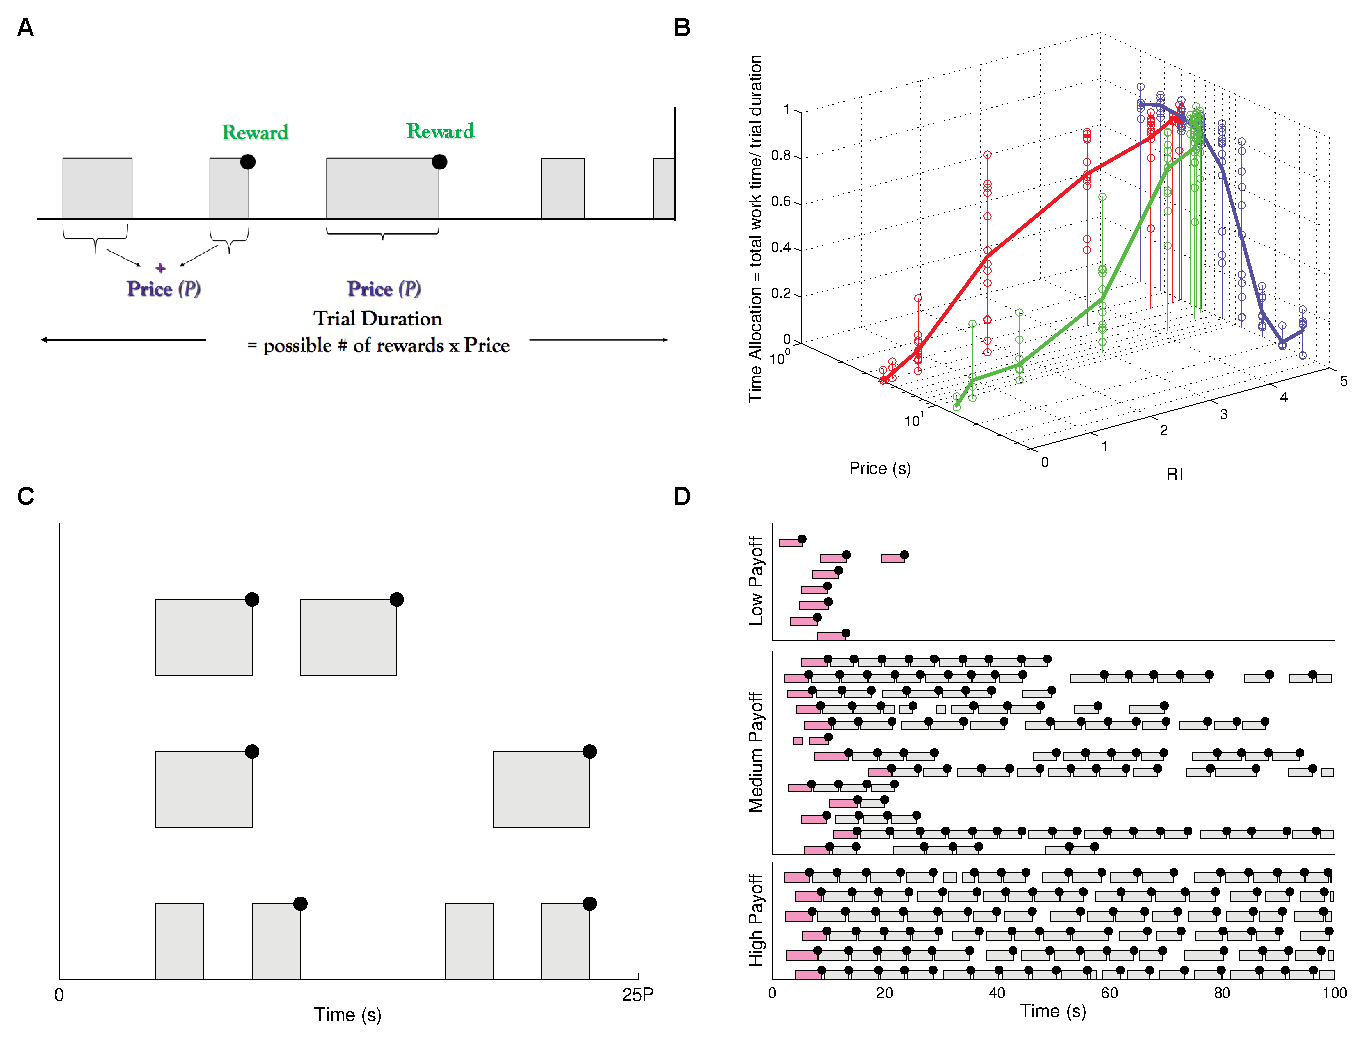
\includegraphics[width=\textwidth]{Fig1}}
\caption{(Colour online) \textbf{Task and key features of the
 data.} \\
 A) Cumulative handling time (CHT) task. Grey bars denote work
(depressing a lever), white gaps show leisure. The subject must
 accumulate work up to a total period of time called the
\emph{price} ($P$) in order to obtain a single reward (black dot) of subjective reward
intensity $RI$. The trial duration is $25\times \mathrm{price}$ (plus
$2$s each time the price is attained, during which the lever is retracted so it cannot
work; not shown).
}
\label{fig:task_data}
\end{figure}

\begin{figure}[ht] 
\widefigure{\fullpagewidth}{Fig1}
\caption{(Colour online) \textbf{Task and key features of the
 data.} \\
A) Cumulative handling time (CHT) task. Grey bars denote work
(depressing a lever), white gaps show leisure. The subject must
accumulate work up to a total period of time called the
\emph{price} ($P$) in order to obtain a single reward (black dot) of subjective reward
intensity $RI$. The trial duration is $25\times \mathrm{price}$ (plus
$2$s each time the price is attained, during which the lever is retracted so it cannot
work; not shown).
}
\label{newfig:task_data}
\end{figure}

\clearpage
\section{Sample tables}

\begin{table}[!ht]
\caption{Time of the Transition Between Phase 1 and Phase 2$^{a}$}
\label{tab:label}
\centering
\begin{tabular}{lc}
\hline
 Run  & Time (min)  \\
\hline
  $l1$  & 260   \\
  $l2$  & 300   \\
  $l3$  & 340   \\
  $h1$  & 270   \\
  $h2$  & 250   \\
  $h3$  & 380   \\
  $r1$  & 370   \\
  $r2$  & 390   \\
\hline
\multicolumn{2}{l}{$^{a}$Table note text here.}
\end{tabular}
\end{table}

\begin{table}[ht]
\widecaption{Sample table taken from [treu03]\label{tbl-1}}
\begin{widetable}
\advance\tabcolsep-1pt
\small
\begin{tabular}{ccrrccccccccc}
\hline
\bf 
POS &\bf  chip &\multicolumn1c{\bf ID} &\multicolumn1c{\bf X}
&\multicolumn1c{\bf Y} &\bf
RA &\bf DEC &\bf IAU$\pm$ $\delta$ IAU &\bf
IAP1$\pm$ $\delta$ IAP1 &\bf IAP2 $\pm$ $\delta$
IAP2 &\bf star &\bf E &\bf Comment\\
\hline
0 & 2 & 1 & 1370.99 & 57.35\rlap{$^a$}    &   6.651120 &  17.131149 &
21.344$\pm$0.006\rlap{$^b$}  & 2 4.385$\pm$0.016 & 23.528$\pm$0.013 & 0.0 & 9 & -    \\
0 & 2 & 2 & 1476.62 & 8.03     &   6.651480 &  17.129572 & 21.641$\pm$0.005  & 2 3.141$\pm$0.007 & 22.007$\pm$0.004 & 0.0 & 9 & -    \\
0 & 2 & 3 & 1079.62 & 28.92    &   6.652430 &  17.135000 & 23.953$\pm$0.030  & 2 4.890$\pm$0.023 & 24.240$\pm$0.023 & 0.0 & - & -    \\
0 & 2 & 4 & 114.58  & 21.22    &   6.655560 &  17.148020 & 23.801$\pm$0.025  & 2 5.039$\pm$0.026 & 24.112$\pm$0.021 & 0.0 & - & -    \\
0 & 2 & 5 & 46.78   & 19.46    &   6.655800 &  17.148932 & 23.012$\pm$0.012  & 2 3.924$\pm$0.012 & 23.282$\pm$0.011 & 0.0 & - & -    \\
0 & 2 & 6 & 1441.84 & 16.16    &   6.651480 &  17.130072 & 24.393$\pm$0.045  & 2 6.099$\pm$0.062 & 25.119$\pm$0.049 & 0.0 & - & -    \\
0 & 2 & 7 & 205.43  & 3.96     &   6.655520 &  17.146742 & 24.424$\pm$0.032  & 2 5.028$\pm$0.025 & 24.597$\pm$0.027 & 0.0 & - & -    \\
0 & 2 & 8 & 1321.63 & 9.76     &   6.651950 &  17.131672 &
22.189$\pm$0.011  & 2 4.743$\pm$0.021 & 23.298$\pm$0.011 & 0.0 & 4 &
edge \\
\hline
\multicolumn{13}{l}{%
Table 2 is published in its entirety in the electronic
edition of the {\it Astrophysical Journal}.}\\[3pt]
\multicolumn{13}{l}{%
$^a$ Sample footnote for table 2.}\\[3pt]
\multicolumn{13}{l}{%
$^b$ Another sample footnote for table 2.}
\end{tabular}
\end{widetable}
\end{table}

\begin{table}[p]
\rotatebox{90}{\vbox{\hsize=\textheight
\caption{Here is a caption for a table that is found in landscape
mode.}
\begin{tabular}{ccrrccccccccc}
\hline
\bf 
POS &\bf  chip &\multicolumn1c{\bf ID} &\multicolumn1c{\bf X}
&\multicolumn1c{\bf Y} &\bf
RA &\bf DEC &\bf IAU$\pm$ $\delta$ IAU &\bf
IAP1$\pm$ $\delta$ IAP1 &\bf IAP2 $\pm$ $\delta$
IAP2 &\bf star &\bf E &\bf Comment\\
\hline
0 & 2 & 1 & 1370.99 & 57.35\rlap{$^a$}    &   6.651120 &  17.131149 &
21.344$\pm$0.006\rlap{$^b$}  & 2 4.385$\pm$0.016 & 23.528$\pm$0.013 & 0.0 & 9 & -    \\
0 & 2 & 2 & 1476.62 & 8.03     &   6.651480 &  17.129572 & 21.641$\pm$0.005  & 2 3.141$\pm$0.007 & 22.007$\pm$0.004 & 0.0 & 9 & -    \\
0 & 2 & 3 & 1079.62 & 28.92    &   6.652430 &  17.135000 & 23.953$\pm$0.030  & 2 4.890$\pm$0.023 & 24.240$\pm$0.023 & 0.0 & - & -    \\
0 & 2 & 4 & 114.58  & 21.22    &   6.655560 &  17.148020 & 23.801$\pm$0.025  & 2 5.039$\pm$0.026 & 24.112$\pm$0.021 & 0.0 & - & -    \\
0 & 2 & 5 & 46.78   & 19.46    &   6.655800 &  17.148932 & 23.012$\pm$0.012  & 2 3.924$\pm$0.012 & 23.282$\pm$0.011 & 0.0 & - & -    \\
0 & 2 & 6 & 1441.84 & 16.16    &   6.651480 &  17.130072 & 24.393$\pm$0.045  & 2 6.099$\pm$0.062 & 25.119$\pm$0.049 & 0.0 & - & -    \\
0 & 2 & 7 & 205.43  & 3.96     &   6.655520 &  17.146742 & 24.424$\pm$0.032  & 2 5.028$\pm$0.025 & 24.597$\pm$0.027 & 0.0 & - & -    \\
0 & 2 & 8 & 1321.63 & 9.76     &   6.651950 &  17.131672 &
22.189$\pm$0.011  & 2 4.743$\pm$0.021 & 23.298$\pm$0.011 & 0.0 & 4 &
edge \\
\hline
\multicolumn{13}{l}{%
Table 2 is published in its entirety in the electronic
edition of the {\it Astrophysical Journal}.}\\[3pt]
\multicolumn{13}{l}{%
$^a$ Sample footnote for table 2.}\\[3pt]
\multicolumn{13}{l}{%
$^b$ Another sample footnote for table 2.}
\end{tabular}
}}
\end{table}
\clearpage


\vglue 3in
Example of table continuing over pages:


\begin{center}
\begin{longtable}{ccc@{}}
\caption{ApJ costs from 1991 to 2013
\label{tab:table}} \\[2pt]
\hline
\bf Year & \bf Subscription & \bf Publication \\
 & \bf cost &\bf charges\\
 & \bf(\$) & \bf (\$/page)\\
\hline
\endfirsthead

\multicolumn3c{Table \thetable, \it continued from previous page.}\\[6pt]
\multicolumn3c{ApJ costs from 1991 to 2013}\\[2pt]
\hline
\bf Year & \bf Subscription & \bf Publication \\
 & \bf cost &\bf charges\\
 & \bf(\$) & \bf (\$/page)\\
\hline
\endhead
\\\hline
\\[-8pt]
\multicolumn{3}{r}{\it Table continued on next page}\\ 
\endfoot

\hline
\endlastfoot

1991 & 600 & 100 \\
1992 & 650 & 105 \\
1993 & 550 & 103 \\
1994 & 450 & 110 \\
1995 & 410 & 112 \\
1996 & 400 & 114 \\
1997 & 525 & 115 \\
1998 & 590 & 116 \\
1999 & 575 & 115 \\
2000 & 450 & 103 \\
2001 & 490 &  90 \\
2002 & 500 &  88 \\
2003 & 450 &  90 \\
2004 & 460 &  88 \\
2005 & 440 &  79 \\
2006 & 350 &  77 \\
2007 & 325 &  70 \\
2008 & 320 &  65 \\
2009 & 190 &  68 \\
2010 & 280 &  70 \\
2011 & 275 &  68 \\
2012 & 150 &  56 \\
2013 & 140 &  55 \\
\end{longtable}
\end{center}

\section{Supportive Information}
Here you enter further sources of information, if desired.

%% A possible entry might be:
% No supportive information is available at this time.


\acknowledgments
Enter your acknowledgments here.

%% ie.,

% The authors thank Laurence Aitchison for fruitful discussions.  RKN
% and PD received funding from the Gatsby Charitable Foundation. Y-AB,
% RBS, KC and PS received funding from Canadian Institutes of Health
% Research grant $MOP74577$,
% Fond de recherche Qu\'{e}bec - Sant\'{e} (Group grant to the Groupe 
% de recherche en neurobiologie comportementale, Shimon Amir, P.I.), and
% Concordia University Research Chair (Tier I). 

\authorcontributions 
Who helped formulate the project, who supplied data, analyses and
experiments, etc.

%% ie.
%% Project was formulated by RKN, PD, PS,
%% based on substantial data, analyses and experiments of Y-AB, KC, RS,
%% PS. RKN, PD formalised the model, RKN implemented and ran the model;
%% RKN analysed the molecular ethogram data; Y-AB formalised and
%% implemented a CTMC model. All authors wrote the manuscript.


%%%%%%%%%%%%%%%%%%%%%%%
%% The bibliography

%% \nocite{*} is used here as a quick way to get every entry  in the .bib file to
%% appear in the bibliography. Normally the bibliography is made using only
%% the bibentries that you cite using \cite{}, or one of the Natbib citation
%% entries, like \citep{}, \citet{} etc.

\nocite{*}
\bibliography{bibsamp}


\appendix

\section{Sample Appendix Section}
We derive the result in Eq. \eqref{eq:analytical_linear}. We consider a linear $C_L(\tau_L+\taupav)=K_L(\tau_L+\taupav)$, and
make two further 
simplifications: (i) the subject does not
engage in leisure in the pre-reward state (and so works for the whole
price when it works); and (ii) \emph{a priori}, arbitrarily long leisure durations are possible
($\lambda=0$).
Then the reward rate in Eq. \eqref{eq:rhoCHT} becomes
\begin{equation}\label{eq:analyticalrho}
\rho^{\pi}= \frac{\vrule height 10pt width0pt RI + K_L \{~ \mathbb{E}[ \tau_L | \textrm{post} ] + \taupav  \} }
     {P +
\mathbb{E}[ \tau_L | \textrm{post} ] +\taupav  } 
\end{equation} 
As discussed in the \emph{Results} section, the probability of engaging in instrumental leisure in the post-reward state is $\pi([L,\tau_L]
~| \textrm{post}) = \exp\left[-\{\beta (\rho^\pi-K_L) 
 \} \tau_L\right]$, which is an exponential distribution with
mean 
\begin{equation}
\mathbb{E}[\tau_L | \textrm{post}]=\frac{1}{\beta (\rho^\pi-K_L) }
\label{eq:analyticaltauL}
\end{equation}  
Re-arranging terms of this equation,
\begin{equation}\label{eq:rhoversion2}
\rho^{\pi}=\frac{1}{\beta ~\mathbb{E}[\tau_L | \textrm{post}]} +K_L 
\end{equation} 
Equating Eqs. \eqref{eq:analyticalrho} and \eqref{eq:rhoversion2} and solving for the mean instrumental leisure duration $\mathbb{E}[\tau_L | \textrm{post}]$, we derive
\begin{equation}
\mathbb{E}[\tau_L | \textrm{post}] = \frac{P+\taupav}{\beta ( RI - K_LP)-1} 
\label{eq:solvedtauL}
\end{equation}
which is the second line of Eq.\eqref{eq:analytical_linear}. This is the mean instrumental leisure duration as long as  $RI - K_LP>1$, and  $\mathbb{E}[\tau_L | \textrm{post}] \rightarrow \infty$ otherwise. When the former condition holds, we may
substitute Eq. \eqref{eq:solvedtauL} into Eq. \eqref{eq:analyticalrho} and solve for $\rho^{\pi}$
\begin{figure}
\widefigure{\fullpagewidth}{Fig1}
\caption{Sample Appendix Caption}
\end{figure}

\newpage

\section{Making Your Bibliography for an Open Mind Article}
{\it Open Mind} uses the APA author-date  bibliography style,
apacite.bst. For more
information on apacite, for examples in how to make your .bib file and more, see:\\
\href{http://mirror.jmu.edu/pub/CTAN/biblio/bibtex/contrib/apacite/apacite.pdf}
{http://mirror.jmu.edu/pub/CTAN/biblio/bibtex/contrib/apacite/apacite.pdf}

\noindent
(In spite of the mention of apacite cite commands, please use only
Natbib commands for in text citations, as shown above.)

\subsection{BibTeX}
You will need to use BibTeX to form your bibliography; typing in the
references would be
a huge and unpleasant task. Look at the openmindsample.bbl file and you'll see why
typing in the bibitems would be difficult. 

For a good basic introduction to using BibTeX, see
\href{https://www.economics.utoronto.ca/osborne/latex/BIBTEX.HTM}
{https://www.economics.utoronto.ca/osborne/latex/BIBTEX.HTM}

When you use BibTeX, the form of the bibliography will be correct. You
don't need to supply a bibliography style, since that is built into
the stjour.cls file.

\end{document}

